\documentclass[12pt,a4paper]{report}
\usepackage{textcomp}
\setlength{\headheight}{13.59999pt}
\usepackage{tocloft}

% ─── Packages ───────────────────────────────────────────────────────────────
\usepackage[top=1in, bottom=1in, left=1.25in, right=1in]{geometry}
\usepackage{graphicx}
\usepackage{amsmath, amssymb}
\usepackage{booktabs}
\usepackage{array}
\usepackage{longtable}
\usepackage{setspace}
\usepackage{parskip}
\usepackage{titlesec}
\usepackage{fancyhdr}
\usepackage{hyperref}
\usepackage{cite}
\usepackage{enumitem}
\usepackage{caption}
\usepackage{subcaption}
\usepackage{float}
\usepackage{xcolor}
\usepackage{microtype}
\usepackage{tikz}
\usepackage{pgfplots}
\pgfplotsset{compat=1.18}
\usepackage{pgfgantt}
\usetikzlibrary{shapes.geometric, arrows.meta, positioning, fit, backgrounds, calc}
\usepackage{colortbl}
\usepackage{multirow}
\usepackage{tabularx}

% ─── Hyperref setup ─────────────────────────────────────────────────────────
\hypersetup{
    colorlinks=true,
    linkcolor=black,
    citecolor=black,
    urlcolor=blue,
    pdftitle={Open-Set Malware Traffic Classification Using 1D-CNNs and JA4 Fingerprinting},
    pdfauthor={Khwopa College of Engineering}
}

% ─── Typography ──────────────────────────────────────────────────────────────
\onehalfspacing
\setlength{\parindent}{0pt}
\setlength{\parskip}{5pt}
\raggedbottom

% ─── Chapter/section formatting ─────────────────────────────────────────────
\titleformat{\chapter}[block]{\large\bfseries\centering}{Chapter \thechapter}{1em}{}
\titleformat{\section}{\normalsize\bfseries}{\thesection}{1em}{}
\titleformat{\subsection}{\normalsize\bfseries}{\thesubsection}{1em}{}
\titlespacing*{\chapter}{0pt}{12pt}{6pt}
\titlespacing*{\section}{0pt}{8pt}{4pt}
\titlespacing*{\subsection}{0pt}{6pt}{3pt}

% ─── Header/footer ───────────────────────────────────────────────────────────
\pagestyle{fancy}
\fancyhf{}
\cfoot{\thepage}
\renewcommand{\headrulewidth}{0pt}

% ─── List / float spacing ────────────────────────────────────────────────────
\setlist[enumerate]{topsep=2pt, itemsep=2pt, parsep=0pt}
\setlist[itemize]{topsep=2pt, itemsep=2pt, parsep=0pt}
\setlength{\floatsep}{6pt}
\setlength{\textfloatsep}{8pt}
\setlength{\intextsep}{4pt}

% ─── TikZ styles ────────────────────────────────────────────────────────────
\tikzset{
  block/.style={rectangle, draw, fill=blue!10, rounded corners,
                text width=2.8cm, text centered, minimum height=1cm, font=\small},
  wideblock/.style={rectangle, draw, fill=blue!10, rounded corners,
                text width=3.8cm, text centered, minimum height=1cm, font=\small},
  decision/.style={diamond, draw, fill=orange!20, text width=2.2cm,
                   text centered, inner sep=0pt, font=\small},
  arrow/.style={-{Stealth[length=2mm]}, thick},
  greenblock/.style={rectangle, draw, fill=green!15, rounded corners,
                text width=2.8cm, text centered, minimum height=1cm, font=\small},
  redblock/.style={rectangle, draw, fill=red!15, rounded corners,
                text width=2.8cm, text centered, minimum height=1cm, font=\small},
  % --- Layer-type styles for CNN architecture diagram ---
  convlayer/.style={rectangle, draw=blue!70, fill=blue!15, rounded corners=3pt,
                    text width=3.2cm, text centered, minimum height=0.85cm,
                    font=\small\bfseries},
  normlayer/.style={rectangle, draw=cyan!70, fill=cyan!10, rounded corners=3pt,
                    text width=3.2cm, text centered, minimum height=0.7cm,
                    font=\small},
  poollayer/.style={rectangle, draw=orange!70, fill=orange!12, rounded corners=3pt,
                    text width=3.2cm, text centered, minimum height=0.7cm,
                    font=\small},
  droplayer/.style={rectangle, draw=red!60, fill=red!8, rounded corners=3pt,
                    text width=3.2cm, text centered, minimum height=0.7cm,
                    font=\small},
  denselayer/.style={rectangle, draw=green!60!black, fill=green!12, rounded corners=3pt,
                     text width=3.2cm, text centered, minimum height=0.85cm,
                     font=\small\bfseries},
  inputlayer/.style={rectangle, draw=gray!80, fill=gray!10, rounded corners=3pt,
                     text width=3.2cm, text centered, minimum height=0.85cm,
                     font=\small\bfseries},
  groupbox/.style={rectangle, draw=gray!50, dashed, rounded corners=6pt,
                   inner sep=8pt},
  grouplabel/.style={font=\scriptsize\bfseries, text=gray!70},
  shapelabel/.style={font=\tiny, text=gray!60},
}

% ─────────────────────────────────────────────────────────────────────────────
\begin{document}

\begin{titlepage}
\thispagestyle{empty}
\begin{center}
\Large\textbf{TRIBHUVAN UNIVERSITY}\\[0.2cm]
\Large\textbf{INSTITUTE OF ENGINEERING}\\[0.5cm]


    \large\textbf{Khwopa College Of Engineering}\\
    \normalsize{Libali, Bhaktapur}\\[0.5cm]

    \large\textbf{Department of Computer Engineering}\\[1cm]

    % Logo
    
\includegraphics[width=0.25\textwidth]{logo.jpg}\\[1cm]

    \large\textbf{A PROPOSAL ON}\\[0.3cm]

    \Large\textbf{Open-Set Malware Traffic Classification}\\[0.2cm]
    \Large\textbf{Using 1D-CNNs and JA4 Fingerprinting}\\[0.8cm]

    \large\textbf{BACHELOR OF COMPUTER ENGINEERING}\\[1cm]

    \large\textbf{Submitted by}\\[0.4cm]

    \begin{tabular}{l @{\hspace{1.5cm}} l}
        Prajin Manandhar    & KCE080BCT022 \\[0.2cm]
        Prashamsha Adhikari & KCE080BCT023 \\[0.2cm]
        Sujal Duwal         & KCE080BCT040 \\[0.2cm]
        Savyata Adhikari    & KCE080BCT048 \\[0.2cm]
    \end{tabular}

    \vfill

    Khwopa College Of Engineering\\
    Libali, Bhaktapur\\
    2026

\end{center}


\end{titlepage}


% ═══════════════════════════════════════════════════════════════════════════
%  FRONT MATTER
% ═══════════════════════════════════════════════════════════════════════════
\pagenumbering{roman}

% ─── Abstract ───────────────────────────────────────────────────────────────
\newpage
\chapter*{Abstract}
\addcontentsline{toc}{chapter}{Abstract}

This project proposes an open-set malware traffic classification framework that
combines JA4 TLS fingerprinting with a 1D-Convolutional Neural Network (1D-CNN)
and a softmax confidence-thresholding rejection layer. Operating exclusively on
the unencrypted TLS Client\,Hello---without decrypting any payload---the system
extracts JA4 fingerprints (with automatic JA3 fallback) and encodes them as
fixed-length numerical vectors for classification. Flows without a TLS handshake
are marked \textit{no fingerprint} and excluded from the pipeline.

A softmax cutoff ($\max_c\,\hat{P}(y{=}c|\mathbf{x}) < 0.70 \Rightarrow$
\textit{Unknown Malware}) flags out-of-distribution traffic and routes it to
analysts, eliminating the closed-set fallacy under which novel malware families
are silently misclassified. Training and evaluation are conducted on CIC-IDS\,2017;
the open-set split trains on Emotet and TrickBot and withholds Zeus as the unknown
family. Class imbalance is addressed through inverse-frequency class weighting
rather than synthetic oversampling. Two baselines are compared: Random Forest on
the same JA4 feature vectors and a JA3-CNN. Dropout\,(0.5) and early stopping
mitigate overfitting on the short feature vectors.

\vspace{0.1cm}
\noindent\textbf{Keywords:} Malware Traffic Classification, TLS Fingerprinting,
JA4, 1D-CNN, Open-Set Recognition, Softmax Thresholding, CIC-IDS, Encrypted
Traffic Analysis

% ─── Table of Contents / Lists ──────────────────────────────────────────────
\newpage
\tableofcontents
\listoftables
\listoffigures

\vspace{0.4cm}
\newpage
% ─── List of Abbreviations (alphabetical order) ─────────────────────────────
{\large\bfseries List of Abbreviations}
\addcontentsline{toc}{chapter}{List of Abbreviations}

\vspace{0.15cm}
\begin{tabular}{ll}
\textbf{Abbreviation} & \textbf{Expansion} \\
1D-CNN & One-Dimensional Convolutional Neural Network \\
ALPN   & Application-Layer Protocol Negotiation \\
APT    & Advanced Persistent Threat \\
AUROC  & Area Under the Receiver Operating Characteristic Curve \\
C\&C   & Command and Control \\
CNN    & Convolutional Neural Network \\
DPI    & Deep Packet Inspection \\
EVT    & Extreme Value Theory \\
FAR    & False Acceptance Rate \\
GREASE & Generate Random Extensions And Sustain Extensibility \\
IDS    & Intrusion Detection System \\
OSR    & Open-Set Recognition \\
PCAP   & Packet Capture \\
RF     & Random Forest \\
ReLU   & Rectified Linear Unit \\
SMOTE  & Synthetic Minority Oversampling Technique \\
SNI    & Server Name Indication \\
SOC    & Security Operations Center \\
TLS    & Transport Layer Security \\
\end{tabular}

% ═══════════════════════════════════════════════════════════════════════════
%  MAIN MATTER
% ═══════════════════════════════════════════════════════════════════════════
\pagenumbering{arabic}

% ═══════════════════════════════════════════════════════════════════════════
%  CHAPTER 1 — INTRODUCTION
% ═══════════════════════════════════════════════════════════════════════════
\chapter{Introduction}

\section{Background}

Over 85\,\% of detected cyber threats are now delivered through encrypted
channels~\cite{zscaler2023}. TLS encryption, while essential for user privacy,
also provides malware authors with a reliable operational cloak: once traffic is
encrypted, traditional deep-packet inspection fails entirely. The key insight that
makes detection without decryption possible is that the TLS \textit{negotiation}
phase---the handshake---occurs in plaintext. Every TLS connection begins with a
Client\,Hello message that encodes the client's supported cipher suites, TLS
version, and protocol extensions. These choices are dictated by the underlying TLS
library and remain characteristic across samples of the same software. JA4,
released by FoxIO in 2023~\cite{althouse2023ja4}, formalises this intuition into
a structured, evasion-resistant fingerprinting standard that supersedes JA3 by
sorting cipher suites and handling GREASE values deterministically. 1D-CNNs have
demonstrated strong performance on sequence-structured network data~\cite{wang2017end},
making them a natural classifier for encoded fingerprint vectors.

Despite this progress, the dominant structural flaw in deployed classifiers
remains the \textit{closed-set fallacy}: every test sample is forced into one of
the classes seen during training~\cite{bendale2016openmax}. When a novel malware
family appears in a live network, such systems do not detect it as unknown---they
confidently misclassify it as the most similar known family, creating a critical
false-negative vector that can allow an advanced threat to persist for months.
IBM's Cost of a Data Breach Report 2023 reports an average breach dwell time
of 204 days~\cite{ibm2023breach}, a window largely attributable to this failure.

\section{Problem Statement}

\subsection{Research Gap}

Two compounding weaknesses characterise current encrypted malware detection:

\begin{enumerate}[leftmargin=*, label=\arabic*.]
  \item \textbf{Closed-Set Fallacy.} Deep learning classifiers trained on known
  families cannot flag genuinely unknown traffic. Novel malware is silently
  misclassified as the nearest known family, generating false
  negatives~\cite{bendale2016openmax, opensetmalware2023}.

  \item \textbf{Outdated Feature Standards.} Much prior work relies on JA3,
  which is vulnerable to cipher-suite reordering and GREASE extension
  randomisation. The integration of JA4 with open-set deep learning has not
  been systematically explored in the literature~\cite{althouse2023ja4}.
\end{enumerate}

\subsection{Impact}

Failing to detect unknown encrypted malware allows APTs and botnets to establish
prolonged dwell time inside organisational networks. Overly aggressive classifiers
that force unknown traffic into known categories generate excessive false positives,
overwhelming SOC analysts with alert fatigue and degrading response capability.

\section{Objectives}

The primary objective is to develop an open-set malware traffic classification
system using JA4 fingerprinting and 1D-CNNs that classifies known families
and flags unseen ones without decrypting TLS communications.



\section{Scope}

This project is scoped to the classification of TLS-encrypted network traffic at the flow level, utilizing only unencrypted TLS Client\,Hello handshake metadata parsed from the CIC-IDS\,2017 dataset. The feature extraction phase is limited to generating JA4 fingerprints, with a fallback to JA3 for malformed handshakes. Flows lacking a TLS handshake are marked \textit{no fingerprint} and excluded from the classification pipeline. The classification is performed using a 1D-Convolutional Neural Network, with open-set recognition implemented via a softmax confidence-thresholding layer set at $\theta = 0.70$. Active SSL/TLS decryption, payload inspection, EVT-based OpenMax calibration, live real-time network integration, and IoT or mobile-specific traffic classification are explicitly out of scope.

% ═══════════════════════════════════════════════════════════════════════════
%  CHAPTER 2 — LITERATURE REVIEW
% ═══════════════════════════════════════════════════════════════════════════
\chapter{Literature Review}

Ten representative papers were reviewed across five thematic areas: TLS fingerprinting, deep learning for traffic classification, open-set recognition in network security, class imbalance strategies, and overfitting mitigation for short feature vectors. The literature reviews of these papers are detailed below.

\section{Anderson \& McGrew --- ML for Encrypted Malware (2017)}
This study demonstrated the efficacy of using passive, unencrypted TLS handshake metadata to classify malware traffic. Utilizing a Random Forest classifier on a large, proprietary dataset of network flows, the authors achieved high detection rates by analyzing cipher suites, extensions, and the server name indication (SNI). However, their system was designed strictly under a closed-set assumption, and the static features remain vulnerable to active mimicry by sophisticated attackers who can spoof handshake metadata.

\section{Wang et al. --- End-to-End Encrypted Traffic via 1D-CNN (2017)}
The authors proposed applying deep learning directly to raw network packet data using 1D-CNNs, treating network traffic as a sequence of bytes. This end-to-end method bypassed manual feature engineering and showed superior classification accuracy on the ISCX VPN-nonVPN dataset compared to traditional machine learning baselines. However, processing raw byte sequences is highly resource-intensive and requires deep packet inspection (DPI), and the classification was limited to a closed-set environment.

\section{Bendale \& Boult --- OpenMax (2016)}
This seminal work introduced the OpenMax model to extend deep neural networks to open-set recognition scenarios. OpenMax utilizes Extreme Value Theory (EVT) to calibrate the activation vectors (Meta-Recognition) of correct validation predictions, fitting a Weibull distribution to establish a threshold-based rejection score for unknown classes. Although demonstrated to improve accuracy on image classification (ImageNet), adapting EVT-calibrated OpenMax to network traffic analysis remains a challenging and relatively unexplored area of research.

\section{Sirinam et al. --- TLS Fingerprinting + ML (2018)}
This research investigated the limits of using TLS handshake fingerprinting (focusing on JA3) combined with Random Forest and Support Vector Machine classifiers to identify client applications and detect malware. The evaluation showed that machine learning models could identify applications with high precision based only on Client Hello negotiation metadata. Nevertheless, the study was constrained by closed-set evaluation and relied on the JA3 standard, which is easily bypassed by modern cipher suite randomization techniques.

\section{Liu et al. --- Semi-Supervised Multimodal Malware Detection (2024)}
Focusing on class imbalance and the lack of labeled data, this paper introduced a semi-supervised multimodal deep learning model. Combining a 1D-CNN with autoencoders, the authors achieved an F1-score of 99.41\% on the UNSW-NB15 dataset using a fraction of labeled samples. The primary limitation of this work is its reliance on a closed-set dataset structure, which does not simulate the emergence of novel, unseen malware families.

\section{SPDConv-Enhanced 1D-CNN (2025)}
Published in the IEEE ICIBA proceedings, this paper introduced Space-to-Depth Convolution (SPDConv) blocks into the 1D-CNN architecture to accelerate inference speed on sequential network data. The authors demonstrated that replacing traditional strided convolution and pooling layers with SPDConv blocks minimizes latency on the CIC-IDS dataset without degrading classification accuracy. However, this study did not evaluate open-set scenarios or incorporate TLS fingerprinting.

\section{Burgetov\'{a} et al. --- JA4+ + Flow Features (2025)}
This work examined the synergistic effect of combining the newer JA4+ fingerprinting standard with traditional flow-level statistical features (e.g., packet counts, packet sizes, and durations). Using a hybrid machine learning approach on the CESNET TLS dataset, the authors showed that fusing application-layer fingerprints with transport-layer flow features yields superior classification performance. The study did not explore deep learning architectures or open-set detection.

\section{Liu et al. --- Multi-Modal 1D-CNN (2025)}
The authors designed a multi-modal 1D-CNN framework that takes both raw packet bytes and header flow statistics as input branches, processing them through an encoder-decoder architecture. Tested on USTC-TFC2016 and ISCX datasets, the fused model proved robust against payload obfuscation. The limitation remains its strict closed-set training environment where all test categories are predefined.

\section{L\'{o}pez de Vergara et al. --- JA4+ vs Flow Features (2025)}
This study presented an empirical comparison between the detection capabilities of the JA4+ fingerprinting standard and traditional flow-level statistics (specifically using the MalDIST tool) for encrypted malware classification. The authors concluded that JA4+ is highly competitive, especially for identifying targeted client-side threats, but is limited when malware mimics legitimate browsers, suggesting the need for multi-modal verification or advanced thresholding.

\section{Chen et al. --- OSR for Malware Traffic (2023)}
Published in MDPI Electronics, this paper proposed an uncertainty-aware deep learning framework for open-set network traffic classification. Using predictive uncertainty estimation, the classifier successfully flags unknown traffic flows in proprietary datasets. However, the model does not exploit TLS handshake fingerprinting standards (like JA4 or JA3) and requires complex probability calibration during inference.


Table~\ref{tab:litreview} presents all reviewed papers
in a unified tabular format, followed by the research gap this project addresses.

\clearpage
\begin{longtable}{|>{\scriptsize}p{0.3cm}|
                  >{\scriptsize}p{2.8cm}|
                  >{\scriptsize}p{0.85cm}|
                  >{\scriptsize}p{1.7cm}|
                  >{\scriptsize}p{2.0cm}|
                  >{\scriptsize}p{2.0cm}|
                  >{\scriptsize}p{1.7cm}|}
\caption{Summary of Reviewed Literature (10 Papers)} \label{tab:litreview} \\
\hline
\textbf{\#} & \textbf{Authors / Title} & \textbf{Year} & \textbf{Method} &
\textbf{Dataset} & \textbf{Key Finding} & \textbf{Gap / Limitation} \\
\hline
\endfirsthead
\multicolumn{7}{c}{\tablename\ \thetable{} \textit{(continued)}} \\
\hline
\textbf{\#} & \textbf{Authors / Title} & \textbf{Year} & \textbf{Method} &
\textbf{Dataset} & \textbf{Key Finding} & \textbf{Gap / Limitation} \\
\hline
\endhead
\hline
\multicolumn{7}{r}{\scriptsize\textit{Continued on next page\ldots}}
\endfoot
\hline
\endlastfoot
1 & Anderson \& McGrew --- ML for Encrypted Malware & 2017 & RF + TLS metadata &
Proprietary TLS flows & TLS metadata identifies malware with high confidence &
No open-set; JA3 evasion possible \\[2pt]
2 & Wang et al. --- End-to-end Encrypted Traffic via 1D-CNN & 2017 & 1D-CNN on raw bytes &
ISCX VPN & 1D-CNNs outperform classical methods without feature engineering &
Closed-set only; raw bytes require DPI \\[2pt]
3 & Bendale \& Boult --- OpenMax & 2016 & EVT + OpenMax &
ImageNet & 4.3\% accuracy gain over SoftMax thresholding &
Vision domain; not tested on network traffic \\[2pt]
4 & Sirinam et al. --- TLS Fingerprinting + ML & 2018 & RF + SVM on TLS metadata &
Synthetic captures & Strong detection without payload access &
Closed-set; JA3 only; no 1D-CNN \\[2pt]
5 & Liu et al. --- Semi-Supervised Multimodal Malware Detection & 2024 & 1D-CNN + semi-supervised &
UNSW-NB15, CIC-IDS & 99.51\% accuracy, 99.41\% F1 on UNSW-NB15 &
Closed-set; no fingerprinting standard \\[2pt]
6 & SPDConv-Enhanced 1D-CNN (IEEE ICIBA) & 2025 & SPDConv + 1D-CNN &
CIC-IDS & Lower latency without accuracy loss &
Closed-set; no open-set evaluation \\[2pt]
7 & Burgetov\'{a} et al. --- JA4+ + Flow Features & 2025 & Hybrid JA4+/flow stats &
CESNET TLS dataset & Hybrid outperforms either modality alone &
No deep learning; no open-set \\[2pt]
8 & Liu et al. --- Multi-Modal 1D-CNN & 2025 & Encoder-decoder + 1D-CNN &
USTC-TFC2016, ISCX & High accuracy on encrypted \& unencrypted traffic &
Closed-set; no fingerprinting \\[2pt]
9 & L\'{o}pez de Vergara et al. --- JA4+ vs Flow Features & 2025 & JA4+ vs MalDIST &
Proprietary captures & JA4+ competitive with flow features &
No 1D-CNN; no open-set \\[2pt]
10 & Chen et al. --- OSR for Malware Traffic (MDPI) & 2023 & Uncertainty-aware DL &
Proprietary traffic & Unknown traffic flagged via predictive uncertainty &
No TLS fingerprinting; complex inference \\[2pt]

\end{longtable}

% ═══════════════════════════════════════════════════════════════════════════
%  SECTION 2.15 — THEORETICAL BACKGROUND
% ═══════════════════════════════════════════════════════════════════════════
\section{Theoretical Background}

\subsection{TLS Handshake and the Client Hello}

TLS encrypts application data, but the negotiation phase---the handshake---occurs
in plaintext. At the start of every TLS connection, the client sends a
\textbf{Client\,Hello} containing: the highest TLS version supported; an ordered
list of cipher suites; TLS extension list including key exchange groups and
signature algorithms; and an ALPN value indicating the desired application
protocol (e.g., HTTP/2). These choices are determined by the client's TLS library
configuration, making them highly characteristic per software type. A Windows
binary compiled with OpenSSL 3.x produces a reliably different Client\,Hello
profile from a browser, a Python script, or a Cobalt Strike beacon. CIC-IDS\,2017
PCAP files include TLS flows from both benign HTTPS traffic and botnet
command-and-control sessions. Flows that carry no TLS handshake (pure UDP,
non-TLS TCP, or mid-session captures) are \textbf{skipped} and labelled
\textit{no fingerprint}; TLS handshake coverage is verified and reported as
part of Step 1 of the pipeline.

\subsection{JA4 Fingerprinting and JA3 Fallback}

JA4 was developed by John Althouse at FoxIO in 2023~\cite{althouse2023ja4} as
a direct successor to JA3. Key improvements are:

\begin{enumerate}[leftmargin=*, label=\arabic*.]
  \item \textbf{Sorted fields.} Cipher suites and extensions are sorted before
  hashing, neutralising cipher-stunting evasion.
  \item \textbf{GREASE handling.} Random bytes inserted by browsers are removed,
  preventing unstable fingerprints.
  \item \textbf{Human-readable format.} A JA4 fingerprint has the form
  \newline$\underbrace{t13d}_{a}\underbrace{070600}_{b}\underbrace{\_c50f5591e341}_{c}\underbrace{\_1a3adfbf9c6b}_{d}$,
  
  where part $a$ encodes protocol type and TLS version; part $b$ encodes cipher
  suite and extension counts; and $c$, $d$ are truncated SHA-256 hashes of the
  sorted cipher suite and extension lists respectively.
  \item \textbf{QUIC support.} JA4 works regardless of whether the connection uses
  TCP or QUIC (HTTP/3).
\end{enumerate}

\textbf{JA3 Fallback.} JA4 extraction may fail when a Client\,Hello is malformed
or truncated. In such cases the pipeline falls back to JA3 computation. Both the
JA4 extraction success rate and JA3 fallback rate are reported per malware family
and overall, providing transparency about data quality.

\subsection{1D Convolutional Neural Networks for Sequential Data}

A 1D-CNN applies learned convolutional filters along a single spatial
dimension~\cite{wang2017end}. The formal operation of a single layer is:
\begin{equation}
  y[i] = \sigma\!\left( \sum_{k=0}^{K-1} w[k]\cdot x[i+k] + b \right)
\end{equation}
where $x$ is the input sequence, $w$ is a filter of length $K$, $b$ is bias,
and $\sigma$ is ReLU. Stacking multiple layers allows the network to learn
hierarchical patterns: early layers capture local field correlations (e.g.,
TLS version vs.\ cipher count) while deeper layers capture higher-order
interactions indicative of specific malware families.

\textbf{Overfitting risk.} JA4 vectors are short ($d \approx 20$--$40$
dimensions after encoding). Short inputs combined with a multi-layer backbone
create a high model-capacity-to-input ratio that leads to rapid memorisation.
Two countermeasures are applied: Dropout $p = 0.5$ in the fully-connected
classification head and early stopping on validation loss with patience of
5 epochs~\cite{srivastava2014dropout, prechelt2012early}.

\subsection{Open-Set Recognition: Softmax Confidence Thresholding}

Classical classifiers operate under the closed-set assumption: the softmax output
sums to 1.0 across $N$ known classes, so any input receives a confident assignment.
This project implements the following rejection rule:

\begin{equation}
  \hat{y} =
  \begin{cases}
    \arg\max_c\, \hat{P}(y{=}c|\mathbf{x}) & \text{if } \max_c\, \hat{P}(y{=}c|\mathbf{x}) \geq 0.70 \\
    \textit{Unknown Malware} & \text{if } \max_c\, \hat{P}(y{=}c|\mathbf{x}) < 0.70
  \end{cases}
\end{equation}

If the model's best-guess confidence is below 70\,\%, the flow is flagged as
unknown rather than being forced into an existing label. The threshold $\theta = 0.70$
is the only hyperparameter of the rejection module and can be adjusted by a SOC
analyst without retraining. EVT-calibrated OpenMax~\cite{bendale2016openmax}
offers a more principled rejection boundary but requires Weibull tail fitting on
held-out validation data per known class, which adds calibration complexity that
is not warranted at MVP stage. Chen et al.~\cite{opensetmalware2023} demonstrated
that simple softmax confidence provides meaningful unknown-malware detection when
the known-class training distribution is sufficiently compact.

\subsection{Class Weighting for Imbalanced Training Data}

Real-world malware datasets are heavily skewed. Rather than applying SMOTE---which
interpolates in feature space and can produce JA4 vectors with physically impossible
configurations (e.g., a cipher-suite count inconsistent with any real TLS
implementation)---this project uses inverse-frequency class weighting:
\begin{equation}
  w_c = \frac{N}{C \cdot N_c}
\end{equation}
where $N$ is the total training sample count, $C$ is the number of classes, and
$N_c$ is the count of samples in class $c$. This penalises misclassification of
minority-class flows more heavily during backpropagation, achieving the same
gradient-level upsampling effect without altering the actual data
distribution~\cite{groupreweight2024}.

\section{Research Gap Identified}

The literature review reveals a clear and unaddressed opportunity: no existing
published work combines JA4 fingerprinting, 1D-CNN classification, and an
integrated open-set rejection mechanism in a single pipeline evaluated on a
concrete family-level open-set split. Prior open-set approaches either target
vision domains (rows 3, 13, 14) or lack TLS fingerprinting entirely (rows 10,
15, 16). JA4-based studies are either classification-free (row 18) or closed-set
(rows 7, 9). This project directly addresses that intersection with a lightweight,
reproducible implementation evaluated on a named split: train on Emotet and
TrickBot, test on Zeus as the unknown family.

% ═══════════════════════════════════════════════════════════════════════════
%  CHAPTER 3 — REQUIREMENT ANALYSIS
% ═══════════════════════════════════════════════════════════════════════════
\chapter{Requirement Analysis}

\section{Software Requirements}

\begin{itemize}
  \item \textbf{Language:} Python 3.10+ (Primary development language)
  \item \textbf{Packet Parsing:} Scapy, PyShark, Wireshark (Parse raw PCAP files; extract TLS Client Hello fields)
  \item \textbf{JA4 Extraction:} FoxIO ja4 toolkit (Generate JA4 strings; fall back to JA3 on failure)
  \item \textbf{Deep Learning:} PyTorch 2.x (1D-CNN model definition, training, and inference)
  \item \textbf{Data Processing:} NumPy, pandas, scikit-learn (Feature encoding, class weighting, train/val split)
  \item \textbf{Visualisation:} Matplotlib, seaborn (Confusion matrices, ROC curves, training history)
  \item \textbf{Version Control:} Git, GitHub (Source code management and collaboration)
\end{itemize}

\section{Functional Requirements}

\begin{enumerate}[leftmargin=*, label=\textbf{FR\arabic*.}]
  \item \textbf{PCAP Ingestion.} Accept raw PCAP files; isolate TLS Client\,Hello
  packets. Flows without a TLS handshake are marked \textit{no fingerprint} and
  excluded; TLS coverage is reported per family.

  \item \textbf{JA4 Extraction with JA3 Fallback.} Attempt JA4 extraction first;
  fall back to JA3 on failure. Report JA4 success rate, JA3 fallback rate, and
  discarded flow count per dataset.

  \item \textbf{Feature Encoding.} Tokenise the fingerprint string into a
  fixed-length numerical vector; apply label encoding to categorical fields and
  min-max normalisation (fitted on training split only) to prevent data leakage.

  \item \textbf{Class-Weighted Training.} Train the 1D-CNN with inverse-frequency
  class weights applied to the cross-entropy loss to handle class imbalance
  without generating synthetic flows.

  \item \textbf{Open-Set Detection.} Flag flows with
  $\max_c\,\hat{P}(y{=}c|\mathbf{x}) < 0.70$ as \textit{Unknown Malware}.

  \item \textbf{Result Output.} Emit per-flow predictions including predicted
  class label (or ``Unknown''), confidence score, and the raw JA4/JA3 fingerprint
  in both human-readable and machine-readable (JSON/CSV) formats.
\end{enumerate}

\section{Non-Functional Requirements}

\begin{enumerate}[leftmargin=*, label=\textbf{NF\arabic*.}]
  \item \textbf{Performance.} Inference on a single flow within 10\,ms on
  a standard CPU.
  \item \textbf{Portability.} Runs on Linux, macOS, and Windows.
  \item \textbf{Maintainability.} PEP\,8 style; rejection threshold $\theta$
  adjustable via configuration file without retraining.
  \item \textbf{Privacy.} No post-handshake payload bytes inspected or logged.
  \item \textbf{Reproducibility.} All seeds, splits, and hyperparameters logged
  via MLflow for exact result reproduction.
\end{enumerate}

\section{Feasibility Study}

\subsection{Technical Feasibility}
All required tools are open-source and well-documented. JA4 parsing tools are
available on GitHub under permissive licences. PyTorch provides mature primitives
for 1D-CNN construction. CIC-IDS\,2017 is publicly available and widely used in
the research community. Training on a mid-range GPU (e.g., NVIDIA RTX 3060,
12\,GB VRAM) or free-tier Google Colab is sufficient for the dataset size involved.

\subsection{Economic Feasibility}
All software dependencies are free and open-source. CIC-IDS\,2017 is freely
downloadable. Cloud compute (Google Colab or Kaggle) provides GPU access at minimal
cost.

\subsection{Operational Feasibility}
The trained model can be integrated into existing SOC tools such as Zeek or
Suricata via a plugin layer. Non-technical analysts interact only with output
labels and confidence scores.

% ═══════════════════════════════════════════════════════════════════════════
%  CHAPTER 4 — METHODOLOGY
% ═══════════════════════════════════════════════════════════════════════════
\chapter{Methodology}

\section{Software Development Approach}

The project runs on an Agile life cycle. Work is split into short, time-boxed sprints, and each one ships a working slice of the system rather than holding everything back for a single release at the end. Inside a sprint the team moves through the same short loop, plan, design, develop, test, review, shown in Figure~\ref{fig:agile_lifecycle}, cutting a thin vertical slice through the pipeline from data and modelling out to the surrounding engineering. Every sprint closes with a review and a retrospective: we demo the increment, then re-plan the next sprint around what we just learned.

\begin{figure}[H]
\centering
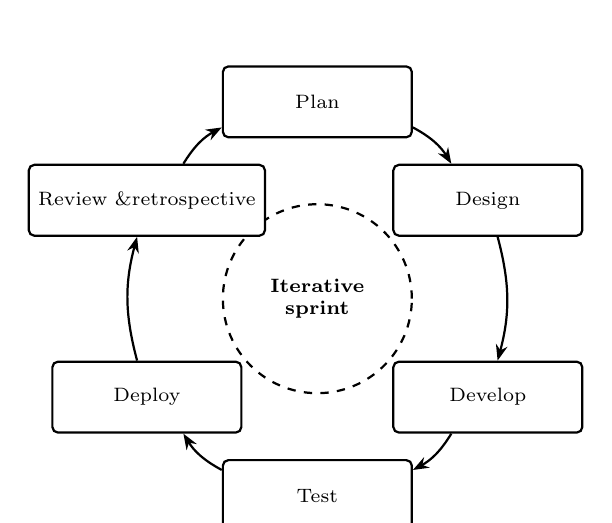
\begin{tikzpicture}[
  node distance=2.2cm,
  stage/.style={rectangle, draw, thick, fill=white, minimum width=2.4cm, minimum height=0.9cm, text centered, font=\scriptsize, rounded corners=2pt},
  arrow/.style={-{Stealth[length=2mm]}, thick}
]
  % Center node
  \draw[dashed, thick] (0,0) circle (1.2cm);
  \node at (0,0) [align=center, font=\scriptsize\bfseries] {Iterative\\sprint};

  % Circular nodes
  \node (plan) at (90:2.5cm) [stage] {Plan};
  \node (design) at (30:2.5cm) [stage] {Design};
  \node (develop) at (330:2.5cm) [stage] {Develop};
  \node (test) at (270:2.5cm) [stage] {Test};
  \node (deploy) at (210:2.5cm) [stage] {Deploy};
  \node (review) at (150:2.5cm) [stage] {Review \&\\retrospective};

  % Curved arrows
  \draw[arrow] (plan) to[bend left=15] (design);
  \draw[arrow] (design) to[bend left=15] (develop);
  \draw[arrow] (develop) to[bend left=15] (test);
  \draw[arrow] (test) to[bend left=15] (deploy);
  \draw[arrow] (deploy) to[bend left=15] (review);
  \draw[arrow] (review) to[bend left=15] (plan);

\end{tikzpicture}
\caption{Agile software development life cycle followed by the project}
\label{fig:agile_lifecycle}
\end{figure}

We picked Agile over a rigid waterfall for a simple reason. The modelling results genuinely change later decisions, the features that end up mattering and the threshold that ends up being safe are not knowable up front and have to be found by experiment. An iterative, adaptive process fits that far better than one plan fixed in advance. So the build is laid out as a run of sprints across the project, as Section~\ref{sec:schedule} sets out.

\section{System Design and Architecture}

\subsection{High-Level System Overview}

The proposed system is a three-stage, decryption-free pipeline:

\begin{enumerate}[leftmargin=*, label=\textbf{Stage \arabic{enumi}:}]
  \item \textbf{JA4 Feature Extraction.} Raw PCAP files are parsed; flows without
  a TLS handshake are marked \textit{no fingerprint}. JA4 is computed for each
  valid Client\,Hello, with automatic JA3 fallback on failure. The fingerprint
  is numerically encoded into a fixed-length vector $\mathbf{f} \in \mathbb{R}^d$.

  \item \textbf{1D-CNN Classification.} The encoded vector is passed through the
  1D-CNN, which produces class probabilities over $N$ known malware families and
  benign traffic.

  \item \textbf{Softmax Confidence Thresholding.} Flows whose maximum class
  probability falls below $\theta = 0.70$ are flagged as \textit{Unknown Malware}
  and routed to analysts; all others receive their predicted label and confidence
  score.
\end{enumerate}

\newpage
\subsection{System Architecture}

Figure~\ref{fig:arch} illustrates the end-to-end pipeline from raw PCAP ingestion
to SOC alert routing. The left branch handles flows that lack a TLS handshake or
where fingerprint extraction fails; the right branch processes successfully
fingerprinted flows through the neural classifier and the rejection layer.

\begin{figure}[H]
\centering
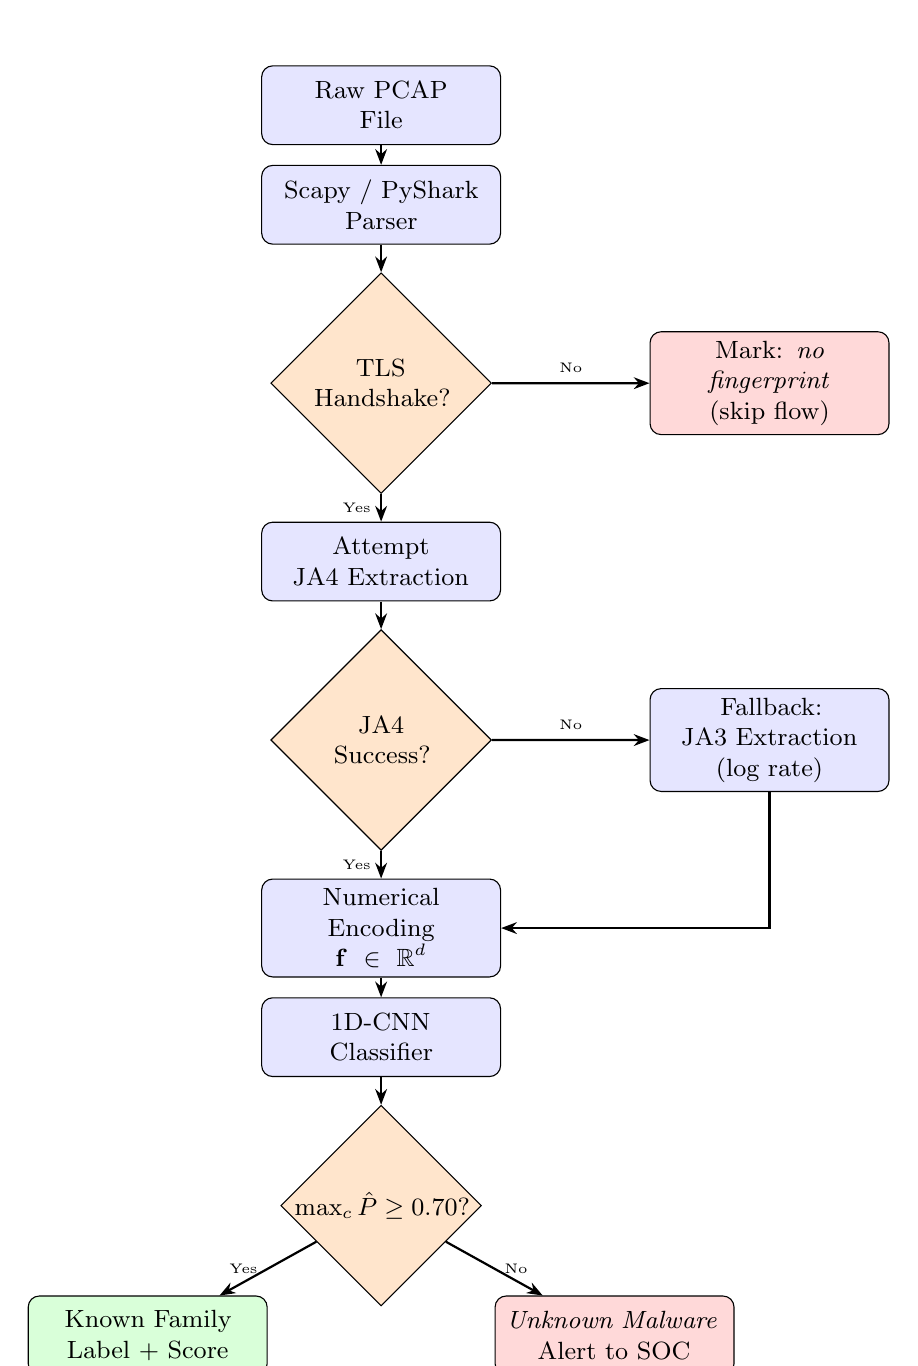
\begin{tikzpicture}[node distance=0.25cm and 0.25cm, scale=0.55]

  \node[block] (pcap) {Raw PCAP\\ File};
  \node[block, below=of pcap] (parse) {Scapy / PyShark\\ Parser};
  \draw[arrow] (pcap) -- (parse);

  \node[decision, below=of parse, yshift=-0.1cm] (tlscheck) {TLS\\ Handshake?};
  \draw[arrow] (parse) -- (tlscheck);

  \node[redblock, right=2.0cm of tlscheck] (nofp)
    {Mark: \textit{no fingerprint}\\ (skip flow)};
  \draw[arrow] (tlscheck) -- node[above, font=\tiny]{No} (nofp);

  \node[block, below=of tlscheck, yshift=-0.1cm] (ja4try) {Attempt\\ JA4 Extraction};
  \draw[arrow] (tlscheck) -- node[left, font=\tiny]{Yes} (ja4try);

  \node[decision, below=of ja4try, yshift=-0.1cm] (ja4ok) {JA4\\ Success?};
  \draw[arrow] (ja4try) -- (ja4ok);

  \node[block, right=2.0cm of ja4ok] (ja3fall)
    {Fallback:\\ JA3 Extraction\\ (log rate)};
  \draw[arrow] (ja4ok) -- node[above, font=\tiny]{No} (ja3fall);

  \node[block, below=of ja4ok, yshift=-0.1cm] (encode)
    {Numerical Encoding\\ $\mathbf{f}\in\mathbb{R}^{d}$};
  \draw[arrow] (ja4ok) -- node[left, font=\tiny]{Yes} (encode);
  \draw[arrow] (ja3fall) |- (encode);

  \node[block, below=of encode] (cnn) {1D-CNN\\ Classifier};
  \draw[arrow] (encode) -- (cnn);

  \node[decision, below=of cnn, yshift=-0.1cm] (thresh) {$\max_c\hat{P} \geq 0.70$?};
  \draw[arrow] (cnn) -- (thresh);

  \node[greenblock, below left=0.5cm and 0.8cm of thresh] (known)
    {Known Family\\ Label + Score};
  \node[redblock, below right=0.5cm and 0.8cm of thresh] (unknown)
    {\textit{Unknown Malware}\\ Alert to SOC};

  \draw[arrow] (thresh) -- node[left, font=\tiny]{Yes} (known);
  \draw[arrow] (thresh) -- node[right, font=\tiny]{No} (unknown);

\end{tikzpicture}
\caption{End-to-end system architecture}
\label{fig:arch}
\end{figure}
\vspace{0.3cm}
\captionsetup{justification=centering}
\small
PCAP ingestion $\to$ TLS handshake check $\to$ JA4 extraction (with JA3 fallback) $\to$ numerical encoding $\to$ 1D-CNN classification $\to$ softmax confidence thresholding. 
Flows scoring below the threshold are routed to the SOC as \textit{Unknown Malware}.

\newpage
\subsection{Use Case Diagram}

The primary actors and system interactions are described in this section. The proposed system has a single external actor, the Security Analyst (or SOC Analyst), who interacts with the classification and alerting pipeline. Figure~\ref{fig:use_case} shows the use cases available to the analyst, which include submitting PCAP files for analysis, viewing classification results and confidence scores, reviewing generated Unknown Malware alerts, adjusting the rejection threshold without model retraining, and exporting the results in CSV or JSON formats.

\begin{figure}[H]
\centering
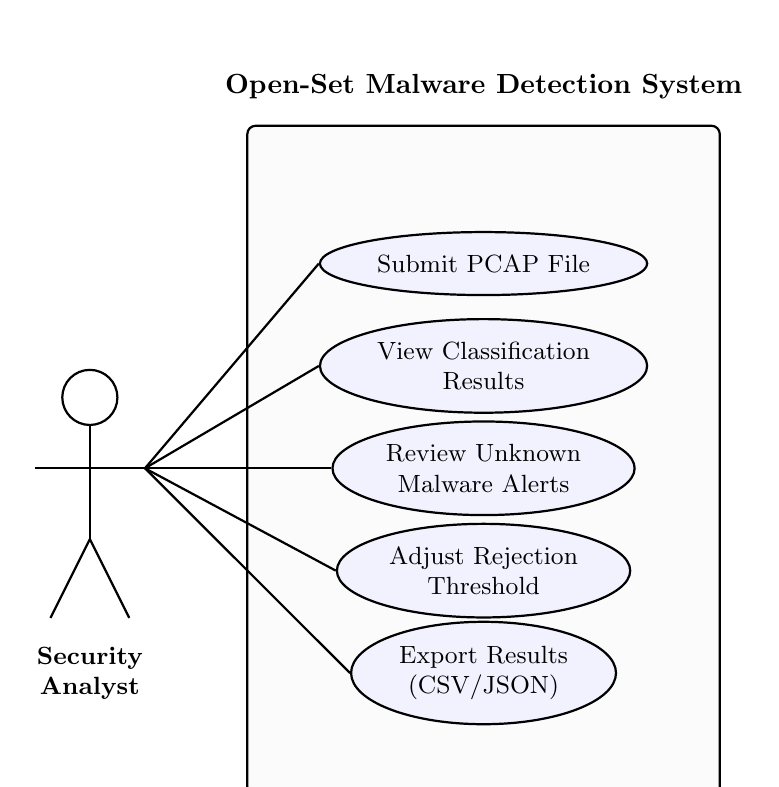
\begin{tikzpicture}[
  actor/.style={draw, circle, minimum size=0.8cm, thick, fill=white},
  usecase/.style={draw, ellipse, minimum width=3.2cm, minimum height=0.8cm, align=center, fill=blue!5, font=\small, thick},
  system/.style={draw, rectangle, minimum width=6cm, minimum height=8.5cm, thick, fill=gray!3, rounded corners=3pt}
]
  % System boundary
  \node[system, label={[font=\bfseries, yshift=0.2cm]above:Open-Set Malware Detection System}] (sys) at (3.5, -3) {};

  % Use Cases
  \node[usecase] (uc1) at (3.5, -0.5) {Submit PCAP File};
  \node[usecase] (uc2) at (3.5, -1.8) {View Classification\\Results};
  \node[usecase] (uc3) at (3.5, -3.1) {Review Unknown\\Malware Alerts};
  \node[usecase] (uc4) at (3.5, -4.4) {Adjust Rejection\\Threshold};
  \node[usecase] (uc5) at (3.5, -5.7) {Export Results\\(CSV/JSON)};

  % Actor: Security Analyst
  % Draw stick figure manually
  \coordinate (head) at (-1.5, -2.2);
  \draw[thick] (head) circle (0.35cm); % Head
  \draw[thick] (-1.5, -2.55) -- (-1.5, -4.0); % Body
  \draw[thick] (-2.2, -3.1) -- (-0.8, -3.1); % Arms
  \draw[thick] (-1.5, -4.0) -- (-2.0, -5.0); % Left leg
  \draw[thick] (-1.5, -4.0) -- (-1.0, -5.0); % Right leg
  \node at (-1.5, -5.7) [align=center, font=\small\bfseries] {Security\\Analyst};

  % Connections
  \draw[thick] (-0.8, -3.1) -- (uc1.west);
  \draw[thick] (-0.8, -3.1) -- (uc2.west);
  \draw[thick] (-0.8, -3.1) -- (uc3.west);
  \draw[thick] (-0.8, -3.1) -- (uc4.west);
  \draw[thick] (-0.8, -3.1) -- (uc5.west);

\end{tikzpicture}
\caption{Use case diagram of the proposed system}
\label{fig:use_case}
\end{figure}
\newpage
\subsection{Block Diagram}

The system block diagram illustrates the major functional blocks of the open-set malware traffic classification pipeline. Figure~\ref{fig:block_diagram} shows the end-to-end component layout. Raw network packets are first ingested and filtered in the packet parser block. The TLS handshakes are then forwarded to the JA4 extraction block, which handles fingerprinting and fallback logic. The generated numeric feature vectors are processed by the 1D-CNN classifier block, and finally, the softmax confidence-thresholding block determines whether to assign a known family label or route the flow as an unknown malware alert.

\begin{figure}[H]
\centering
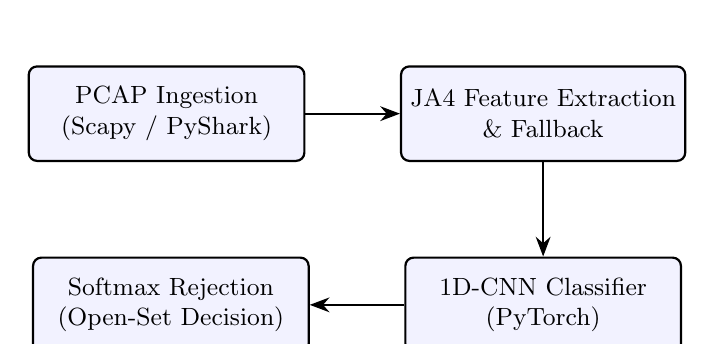
\begin{tikzpicture}[
  block/.style={draw, rectangle, minimum width=3.5cm, minimum height=1.2cm, align=center, fill=blue!5, font=\small, thick, rounded corners=3pt},
  arrow/.style={-{Stealth[length=2.5mm]}, thick}
]
  \node (pcap) [block] {PCAP Ingestion \\ (Scapy / PyShark)};
  \node (prep) [block, right=1.2cm of pcap] {JA4 Feature Extraction \\ \& Fallback};
  \node (cnn) [block, below=1.2cm of prep] {1D-CNN Classifier \\ (PyTorch)};
  \node (rej) [block, left=1.2cm of cnn] {Softmax Rejection \\ (Open-Set Decision)};

  \draw[arrow] (pcap) -- (prep);
  \draw[arrow] (prep) -- (cnn);
  \draw[arrow] (cnn) -- (rej);
\end{tikzpicture}
\caption{System block diagram of the proposed model}
\label{fig:block_diagram}
\end{figure}

\subsection{Activity Diagram}

The activity diagram describes the sequential workflow and decision paths executed for each network flow in the detection pipeline. As shown in Figure~\ref{fig:activity_diagram}, when a PCAP file is parsed, the system checks if a TLS Client Hello is present. Non-TLS flows are immediately skipped and labeled as 'no fingerprint'. For TLS-bearing flows, the system attempts JA4 extraction. If JA4 fails due to malformed packets, it falls back to JA3 extraction. The resulting fingerprint is encoded into a normalised feature vector and passed to the 1D-CNN. If the model's prediction confidence meets or exceeds the threshold of 0.70, it outputs the known malware family or benign label; otherwise, it triggers an 'Unknown Malware' alert for SOC analyst review.

\begin{figure}[H]
\centering
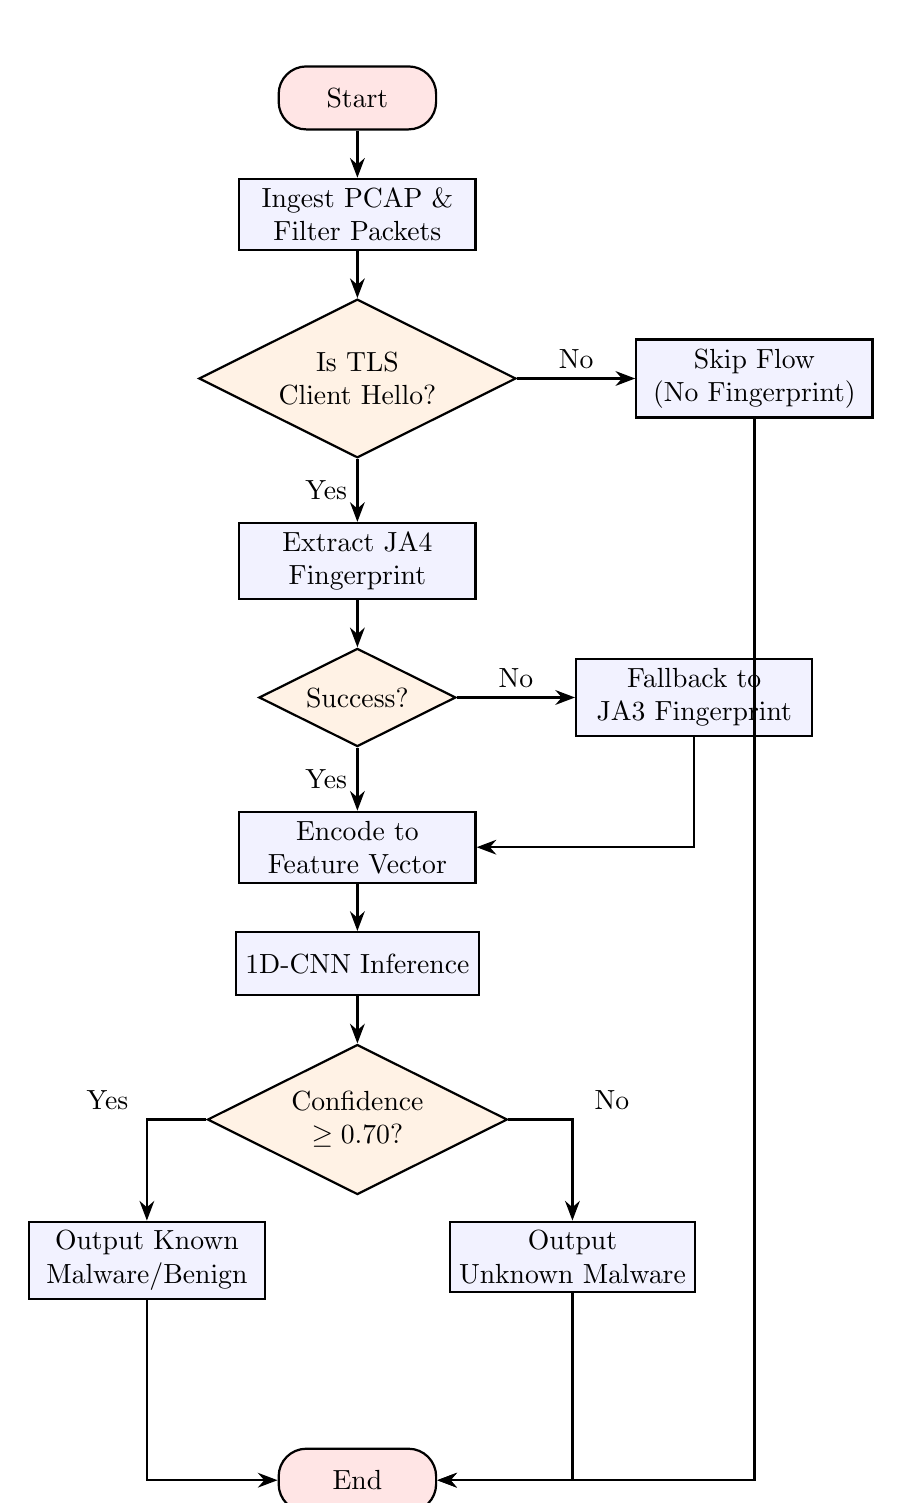
\begin{tikzpicture}[
  startstop/.style={draw, rectangle, rounded corners=10pt, minimum width=2cm, minimum height=0.8cm, align=center, fill=red!10, thick},
  process/.style={draw, rectangle, minimum width=3cm, minimum height=0.8cm, align=center, fill=blue!5, thick},
  decision/.style={draw, diamond, aspect=2, minimum width=2.5cm, minimum height=1cm, align=center, fill=orange!10, thick},
  arrow/.style={-{Stealth[length=2.5mm]}, thick}
]
  \node (start) [startstop] {Start};
  \node (ingest) [process, below=0.6cm of start] {Ingest PCAP \&\\Filter Packets};
  \node (dec1) [decision, below=0.6cm of ingest] {Is TLS\\Client Hello?};
  \node (skip) [process, right=1.5cm of dec1] {Skip Flow\\(No Fingerprint)};
  \node (ja4) [process, below=0.8cm of dec1] {Extract JA4\\Fingerprint};
  \node (dec2) [decision, below=0.6cm of ja4] {Success?};
  \node (ja3) [process, right=1.5cm of dec2] {Fallback to\\JA3 Fingerprint};
  \node (encode) [process, below=0.8cm of dec2] {Encode to\\Feature Vector};
  \node (cnn) [process, below=0.6cm of encode] {1D-CNN Inference};
  \node (dec3) [decision, below=0.6cm of cnn] {Confidence\\$\ge 0.70$?};
  \node (known) [process, below left=0.8cm and 0.2cm of dec3] {Output Known\\Malware/Benign};
  \node (unknown) [process, below right=0.8cm and 0.2cm of dec3] {Output\\Unknown Malware};
  \node (end) [startstop, below=3.2cm of dec3] {End};

  \draw[arrow] (start) -- (ingest);
  \draw[arrow] (ingest) -- (dec1);
  \draw[arrow] (dec1) -- node[left] {Yes} (ja4);
  \draw[arrow] (dec1) -- node[above] {No} (skip);
  \draw[arrow] (ja4) -- (dec2);
  \draw[arrow] (dec2) -- node[left] {Yes} (encode);
  \draw[arrow] (dec2) -- node[above] {No} (ja3);
  \draw[arrow] (ja3) |- (encode);
  \draw[arrow] (encode) -- (cnn);
  \draw[arrow] (cnn) -- (dec3);
  \draw[arrow] (dec3) -| node[above, xshift=-0.5cm] {Yes} (known);
  \draw[arrow] (dec3) -| node[above, xshift=0.5cm] {No} (unknown);
  \draw[arrow] (known) |- (end);
  \draw[arrow] (unknown) |- (end);
  \draw[arrow] (skip) |- (end);
\end{tikzpicture}
\caption{Activity diagram of the proposed classification process}
\label{fig:activity_diagram}
\end{figure}
\newpage
\subsection{Proposed 1D-CNN Architecture}

Two convolutional blocks (rather than three) are used to keep the model
appropriately sized for the short input vector and reduce the risk of
over-parameterisation. Figure~\ref{fig:cnn_arch} illustrates the architecture.

\begin{figure}[H]
\centering
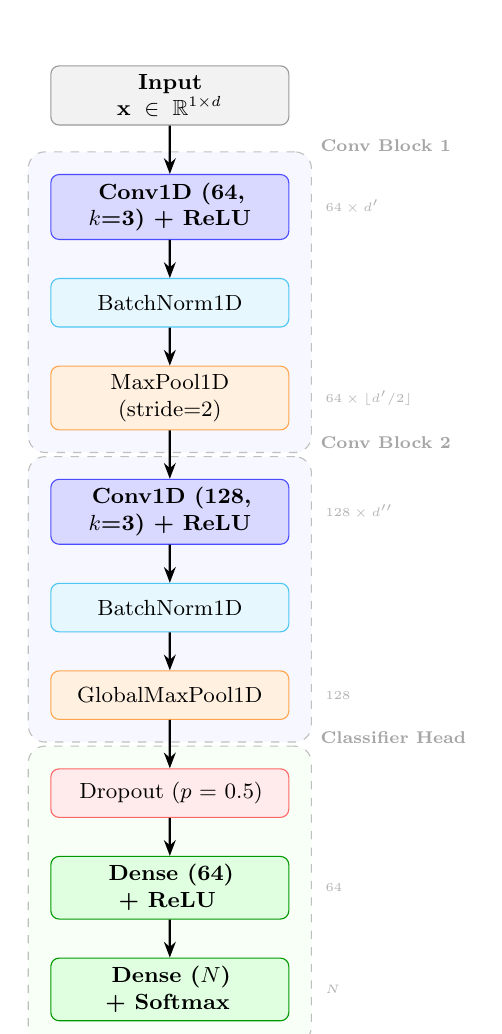
\begin{tikzpicture}[node distance=0.55cm, scale=0.88, transform shape]
  % --- Input ---
  \node[inputlayer] (in) {Input\\$\mathbf{x} \in \mathbb{R}^{1 \times d}$};

  % --- Conv Block 1 ---
  \node[convlayer, below=0.7cm of in] (c1) {Conv1D (64, $k$=3) + ReLU};
  \node[normlayer, below=of c1] (bn1) {BatchNorm1D};
  \node[poollayer, below=of bn1] (mp1) {MaxPool1D (stride=2)};

  % --- Conv Block 2 ---
  \node[convlayer, below=0.7cm of mp1] (c2) {Conv1D (128, $k$=3) + ReLU};
  \node[normlayer, below=of c2] (bn2) {BatchNorm1D};
  \node[poollayer, below=of bn2] (gmp) {GlobalMaxPool1D};

  % --- Classifier Head ---
  \node[droplayer, below=0.7cm of gmp] (drop) {Dropout ($p$ = 0.5)};
  \node[denselayer, below=of drop] (fc1) {Dense (64) + ReLU};
  \node[denselayer, below=of fc1] (out) {Dense ($N$) + Softmax};

  % --- Arrows ---
  \draw[arrow] (in) -- (c1);
  \draw[arrow] (c1) -- (bn1);
  \draw[arrow] (bn1) -- (mp1);
  \draw[arrow] (mp1) -- (c2);
  \draw[arrow] (c2) -- (bn2);
  \draw[arrow] (bn2) -- (gmp);
  \draw[arrow] (gmp) -- (drop);
  \draw[arrow] (drop) -- (fc1);
  \draw[arrow] (fc1) -- (out);

  % --- Group boxes ---
  \begin{scope}[on background layer]
    \node[groupbox, fill=blue!3,
          fit=(c1)(bn1)(mp1),
          label={[grouplabel]above right:{Conv Block 1}}] {};
    \node[groupbox, fill=blue!3,
          fit=(c2)(bn2)(gmp),
          label={[grouplabel]above right:{Conv Block 2}}] {};
    \node[groupbox, fill=green!3,
          fit=(drop)(fc1)(out),
          label={[grouplabel]above right:{Classifier Head}}] {};
  \end{scope}

  % --- Tensor shape annotations ---
  \node[shapelabel, right=0.4cm of c1]  {$64 \times d'$};
  \node[shapelabel, right=0.4cm of mp1] {$64 \times \lfloor d'/2 \rfloor$};
  \node[shapelabel, right=0.4cm of c2]  {$128 \times d''$};
  \node[shapelabel, right=0.4cm of gmp] {128};
  \node[shapelabel, right=0.4cm of fc1] {64};
  \node[shapelabel, right=0.4cm of out] {$N$};
\end{tikzpicture}
\caption{Proposed 1D-CNN Architecture. Colour key: {\color{blue!70}\rule{0.6em}{0.6em}}~Convolution,
{\color{cyan!70}\rule{0.6em}{0.6em}}~Normalisation,
{\color{orange!70}\rule{0.6em}{0.6em}}~Pooling,
{\color{red!60}\rule{0.6em}{0.6em}}~Regularisation,
{\color{green!60!black}\rule{0.6em}{0.6em}}~Dense.}
\label{fig:cnn_arch}
\end{figure}

The 64 $\rightarrow$ 128 filter progression is deliberately conservative given
the short JA4 input. Dropout $p = 0.5$ at the fully-connected layer follows
the recommendation of Srivastava et al.~\cite{srivastava2014dropout}.
GlobalMaxPool collapses the spatial dimension rather than Flatten, reducing the
parameter count and adding mild translation invariance. BatchNorm after each
convolutional layer accelerates convergence and reduces sensitivity to
initialisation.

\newpage
\section{Open-Set Detection Workflow}

Figure~\ref{fig:openset} illustrates the family-level open-set evaluation
scenario. The model is trained exclusively on Emotet and TrickBot flows; Zeus
flows are withheld entirely from training and presented only at test time.
A correct open-set classifier will assign Zeus flows a maximum confidence below
0.70 and flag them as \textit{Unknown Malware} rather than forcing them into
the Emotet or TrickBot class.

\vspace{0.3cm}
\begin{figure}[H]
\centering
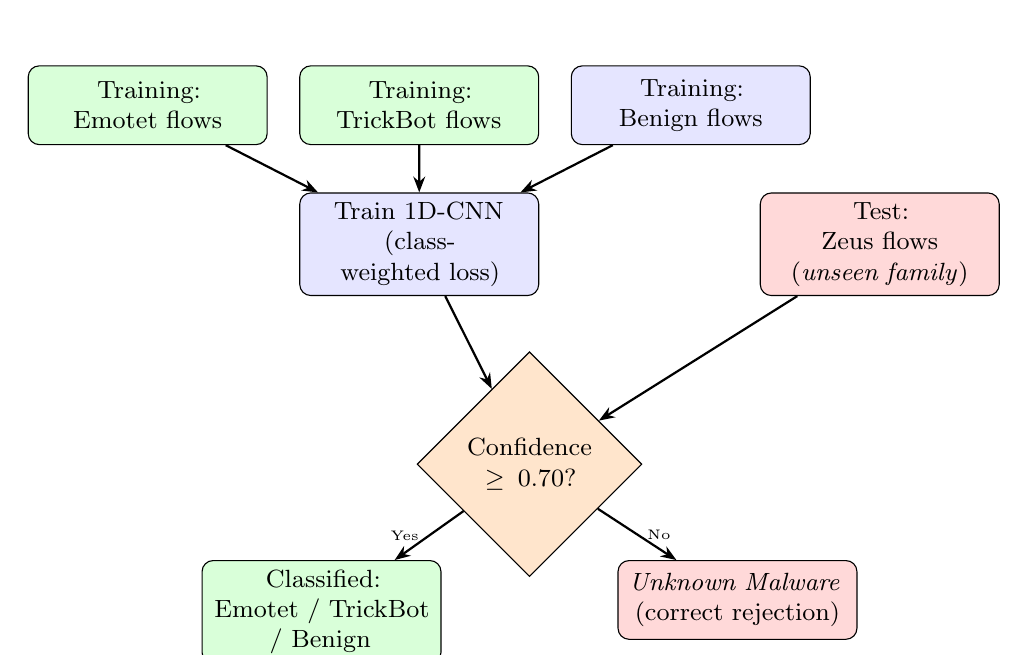
\begin{tikzpicture}[node distance=0.25cm and 0.5cm, scale=0.6]
  \node[greenblock] (tr1) {Training:\\ Emotet flows};
  \node[greenblock, right=0.4cm of tr1] (tr2) {Training:\\ TrickBot flows};
  \node[block, right=0.4cm of tr2] (ben) {Training:\\ Benign flows};

  \node[block, below=0.6cm of tr2] (cnn2)
    {Train 1D-CNN\\ (class-weighted loss)};
  \draw[arrow] (tr1) -- (cnn2);
  \draw[arrow] (tr2) -- (cnn2);
  \draw[arrow] (ben) -- (cnn2);

  \node[redblock, right=2.8cm of cnn2] (zeus)
    {Test:\\ Zeus flows\\ (\textit{unseen family})};

  \node[decision, below=0.7cm of cnn2, xshift=1.4cm] (conf)
    {Confidence\\ $\geq 0.70$?};
  \draw[arrow] (cnn2) -- (conf);
  \draw[arrow] (zeus) -- (conf);

  \node[greenblock, below left=0.5cm and 0.4cm of conf] (fp)
    {Classified:\\ Emotet / TrickBot\\ / Benign};
  \node[redblock, below right=0.5cm and 0.4cm of conf] (uk)
    {\textit{Unknown Malware}\\ (correct rejection)};

  \draw[arrow] (conf) -- node[left, font=\tiny]{Yes} (fp);
  \draw[arrow] (conf) -- node[right, font=\tiny]{No} (uk);
\end{tikzpicture}
\caption{Open-set evaluation protocol}
\label{fig:openset}
\end{figure}
\vspace{0.3cm}
\captionsetup{justification=centering}
\small
The model trains on Emotet and TrickBot flows; Zeus flows are withheld from training entirely and presented at test time as the unknown family. Correct rejections (Zeus flagged as \textit{Unknown}) are true positives for the open-set AUROC metric.
\newpage
\section{Operational Workflow of the System}

Figure~\ref{fig:workflow} presents the complete workflow. Steps 1--5 (left column)
cover data preparation; Steps 6--9 (right column) cover model training, evaluation,
and baseline comparison.

\begin{figure}[H]
\centering
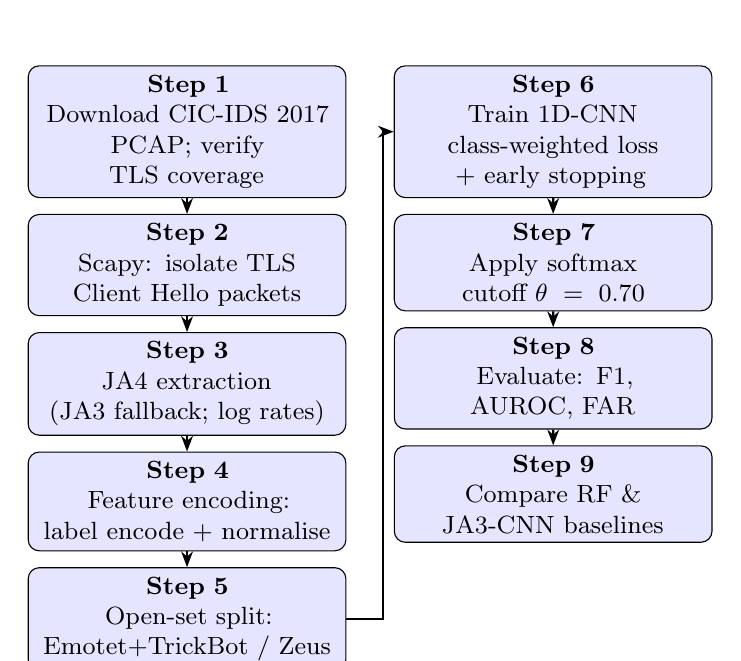
\begin{tikzpicture}[node distance=0.2cm and 0.6cm, scale=0.58]
  \node[wideblock] (s1) {\textbf{Step 1}\\ Download CIC-IDS 2017\\ PCAP; verify TLS coverage};
  \node[wideblock, below=of s1] (s2) {\textbf{Step 2}\\ Scapy: isolate TLS\\ Client Hello packets};
  \node[wideblock, below=of s2] (s3) {\textbf{Step 3}\\ JA4 extraction\\ (JA3 fallback; log rates)};
  \node[wideblock, below=of s3] (s4) {\textbf{Step 4}\\ Feature encoding:\\ label encode + normalise};
  \node[wideblock, below=of s4] (s5) {\textbf{Step 5}\\ Open-set split:\\ Emotet+TrickBot / Zeus};

  \draw[arrow] (s1)--(s2); \draw[arrow] (s2)--(s3);
  \draw[arrow] (s3)--(s4); \draw[arrow] (s4)--(s5);

  \node[wideblock, right=of s1] (s6) {\textbf{Step 6}\\ Train 1D-CNN\\ class-weighted loss\\ + early stopping};
  \node[wideblock, below=of s6] (s7) {\textbf{Step 7}\\ Apply softmax\\ cutoff $\theta = 0.70$};
  \node[wideblock, below=of s7] (s8) {\textbf{Step 8}\\ Evaluate: F1,\\ AUROC, FAR};
  \node[wideblock, below=of s8] (s9) {\textbf{Step 9}\\ Compare RF \&\\ JA3-CNN baselines};

  \draw[arrow] (s6)--(s7); \draw[arrow] (s7)--(s8);
  \draw[arrow] (s8)--(s9);

  \draw[arrow] (s5.east) -- ++(0.8,0) |- (s6.west);
\end{tikzpicture}
\caption{Complete project workflow}
\label{fig:workflow}
\end{figure}
\vspace{0.1cm}
\captionsetup{justification=centering}
\small
Steps~1--5 (left column) cover PCAP acquisition, TLS handshake isolation, JA4 extraction, feature encoding, and open-set splitting. Steps~6--9 (right column) cover 1D-CNN training, softmax thresholding, evaluation, and baseline comparison.

\subsection{Data Collection}
A single dataset is used for all experiments: \textbf{CIC-IDS\,2017} (Canadian Institute for Cybersecurity Intrusion Detection Evaluation Dataset)~\cite{sharafaldin2018cicids}, capturing one week of realistic network traffic (July 3--7, 2017) across multiple attack types including botnet activity. Raw PCAP files are publicly available, allowing genuine JA4 extraction from packet captures rather than pre-computed flow statistics. TLS handshake coverage is verified and reported per malware family; flows lacking a complete handshake are excluded.

\textbf{Open-set split definition.} Training uses all Emotet and TrickBot flows plus a balanced benign sample. Zeus flows are withheld entirely from training and presented only at test time as the unknown family. This makes the split concrete and reproducible: any researcher can replicate it exactly by filtering on the published family labels.

For the step-by-step data collection, the raw PCAP files are downloaded from the Canadian Institute for Cybersecurity repository. The SHA-256 checksums are verified. All PCAP files are scanned to count flows with and without TLS handshakes, reporting TLS coverage per family label. This confirms whether sufficient fingerprint-able traffic exists for each class.

\subsection{Data Preprocessing}
Use Scapy to filter packets matching TLS record type 0x16 (Handshake) with handshake type 0x01 (Client Hello). Flows containing no such packet are marked \textit{no fingerprint} and excluded.

\textbf{Justification:} Non-TLS flows carry no handshake metadata and cannot be fingerprinted; including them as a separate class would confound the classification problem.

\subsection{Feature Engineering}
Apply the FoxIO open-source JA4 toolkit to each extracted Client\,Hello. On failure (malformed or truncated extensions), fall back to JA3 computation. Report: JA4 extraction success rate (per family and overall), JA3 fallback rate, and discarded flow count.

\textbf{Justification:} Reporting these rates is a data-quality transparency requirement. The JA3 fallback ensures maximum flow coverage.

For the feature encoding, we parse each fingerprint string into component fields: TLS version code, cipher-suite count, extension count, ALPN value, sorted cipher-suite hash, sorted extension hash. Apply label encoding to categorical fields, hex-to-integer conversion for hash fields, and min-max normalisation $([0,1])$ fitted on the training split only to prevent data leakage. The result is a fixed-length vector $\mathbf{f} \in \mathbb{R}^d$ per flow.

\subsection{Model Selection}
The 1D-CNN model training is configured with the following parameters:
\begin{itemize}[leftmargin=*]
  \item \textbf{Loss:} Categorical cross-entropy with inverse-frequency class weights.
  \item \textbf{Optimiser:} Adam, initial learning rate $\eta = 10^{-3}$.
  \item \textbf{Regularisation:} Dropout $p = 0.5$ in the FC head.
  \item \textbf{Early stopping:} Halt if validation loss does not improve for 5 consecutive epochs; restore best weights.
  \item \textbf{Batch size:} 64.
\end{itemize}

\textbf{Why class weighting over SMOTE:} SMOTE interpolates between existing minority samples in feature space. For network features (cipher-suite counts, extension lists), interpolated samples can represent TLS configurations that no real software library produces, introducing artefacts that may bias the classifier. Class weighting achieves the same gradient-level upsampling without altering the data distribution~\cite{groupreweight2024}.

\textbf{Why early stopping over grid search + k-fold:} Grid search and 5-fold cross-validation are computationally intensive and statistically unnecessary for a dataset of this size in a four-month undergraduate project. A single 80/10/10 split with early stopping produces reliable model selection.

\subsection{Model Evaluation}
The open-set data split is defined as follows:
\begin{itemize}[leftmargin=*]
  \item \textbf{Training (80\,\%):} Emotet + TrickBot + balanced benign flows.
  \item \textbf{Validation (10\,\%):} Held-out portion of same three classes; used for early stopping and threshold sensitivity analysis.
  \item \textbf{Closed-set test (5\,\%):} Held-out Emotet / TrickBot / Benign flows.
  \item \textbf{Open-set test (5\,\%):} All Zeus flows (entirely withheld from training); correct classifier flags these as \textit{Unknown Malware}.
\end{itemize}

\textbf{Justification:} Withholding an entire named family is the standard methodology for family-level open-set evaluation~\cite{opensetmalware2023}.

For open-set detection, we apply the rejection rule $\theta = 0.70$ to all test flows. A sensitivity analysis over $\theta \in \{0.60, 0.65, 0.70, 0.75, 0.80\}$ is performed to characterise the precision--recall trade-off for the SOC operator.

The performance is evaluated using the following metrics:
\textbf{Closed-set metrics:} Accuracy, Precision, Recall, and F1-Score per class.

\textbf{Open-set metrics:}
\begin{itemize}[leftmargin=*]
  \item \textbf{AUROC:} Area under the ROC curve treating \textit{Unknown Malware} detection as a binary problem (unknown vs.\ known). Perfect open-set score: 1.0.
  \item \textbf{Open-set F1:} F1-score treating correctly rejected Zeus flows as true positives.
  \item \textbf{FAR:} Fraction of Zeus flows incorrectly assigned to a known class.
  \item \textbf{JA4 Extraction Success Rate:} Reported per family.
\end{itemize}

Finally, we evaluate two baselines on the same features and split:
\begin{enumerate}[leftmargin=*, label=\arabic*.]
  \item \textbf{Random Forest (RF):} Scikit-learn RF with 100 trees and class weighting on the same JA4 feature vectors. Open-set rejection is proxied by the fraction of trees voting for the winning class.
  \item \textbf{JA3-CNN:} Identical 1D-CNN architecture trained on JA3 feature vectors, to isolate the contribution of the updated fingerprinting standard.
\end{enumerate}

\textbf{Why not SVM:} SVM scales poorly to tens of thousands of flows (quadratic memory in support vectors) and does not produce well-calibrated probabilities without Platt scaling. Dropping SVM keeps the comparison focused: does JA4 outperform JA3 as a 1D-CNN input, and does the 1D-CNN outperform RF?

\section{Estimated Time Schedule}
\label{sec:schedule}

The project is planned across an eight-week timeline, divided into weekly milestones. Weeks 1--2 cover literature review, dataset download, and JA4 extraction pipeline development. Weeks 3--4 cover JA3 fallback integration, feature encoding, and the open-set data split. Weeks 5--6 cover 1D-CNN training, softmax thresholding implementation, and baseline comparisons. Weeks 7--8 cover evaluation, prototype packaging, and finalizing the project report. Report writing runs continuously throughout all eight weeks to document findings and decisions incrementally. Figure~\ref{fig:gantt} presents the project schedule.

\begin{figure}[H]
\centering
\resizebox{\textwidth}{!}{
\begin{ganttchart}[
    hgrid,
    vgrid,
    x unit=1.2cm,
    y unit title=0.6cm,
    y unit chart=0.5cm,
    title label font=\tiny\bfseries,
    bar label font=\tiny,
    group label font=\tiny\bfseries,
    milestone label font=\tiny\itshape,
    bar height=0.5,
    group right shift=0,
    group top shift=0.4,
    group height=0.25,
    bar/.append style={fill=blue!30, draw=blue!60},
    group/.append style={fill=gray!30, draw=gray!60},
    milestone/.append style={fill=red!60, draw=red!80},
    title height=1
 ]{1}{8}

  % Title rows: Months and Weeks
  \gantttitle{Month 1}{4}
  \gantttitle{Month 2}{4} \\
  \gantttitlelist{1,...,8}{1} \\

  % --- Phase 1: Data Acquisition & Preprocessing ---
  \ganttgroup{Phase 1: Data \& Preprocessing}{1}{4} \\
  \ganttbar{Literature Review}{1}{2} \\
  \ganttbar{Dataset Download \& TLS Verification}{1}{2} \\
  \ganttbar{JA4 Extraction Pipeline}{2}{3} \\
  \ganttbar{JA3 Fallback Integration}{3}{3} \\
  \ganttbar{Feature Encoding}{3}{4} \\
  \ganttbar{Open-set Split (Train/Test)}{4}{4} \\

  % --- Phase 2: Model Development ---
  \ganttgroup{Phase 2: Model Development}{4}{6} \\
  \ganttbar{1D-CNN Training}{4}{5} \\
  \ganttbar{Softmax Thresholding}{5}{5} \\
  \ganttbar{Baseline Implementation (RF, JA3-CNN)}{5}{6} \\

  % --- Phase 3: Evaluation & Reporting ---
  \ganttgroup{Phase 3: Evaluation \& Reporting}{6}{8} \\
  \ganttbar{Evaluation (F1, AUROC, FAR)}{6}{7} \\
  \ganttbar{Baseline Comparison}{7}{7} \\
  \ganttbar{Prototype Packaging}{7}{8} \\
  \ganttbar{Report Writing}{1}{8} \\
  \ganttmilestone{Final Submission}{8}

  % --- Dependencies ---
  \ganttlink{elem2}{elem3}
  \ganttlink{elem3}{elem4}
  \ganttlink{elem5}{elem6}
  \ganttlink{elem8}{elem9}
  \ganttlink{elem9}{elem10}
  \ganttlink{elem12}{elem13}

\end{ganttchart}
}
\caption{Project Gantt Chart (8 Weeks / 2 Months)}
\label{fig:gantt}
\end{figure}

% ═══════════════════════════════════════════════════════════════════════════
%  CHAPTER 5 — EXPECTED RESULTS
% ═══════════════════════════════════════════════════════════════════════════
\chapter{Expected Results}

\begin{enumerate}[leftmargin=*, label=\arabic*.]
  \item \textbf{JA4 extraction pipeline} that processes CIC-IDS\,2017 PCAPs and
  reports per-family JA4 success rates, JA3 fallback rates, and TLS handshake
  coverage, with documented code and unit tests.

  \item \textbf{Trained 1D-CNN} achieving competitive closed-set F1-scores on
  Emotet and TrickBot test splits, benchmarked against RF and JA3-CNN. Based on
  comparable architectures~\cite{liu2024encrypted, spd2025}, F1-scores above
  90\,\% are anticipated for the most prevalent known families.

  \item \textbf{Measurable open-set detection:} the softmax thresholding module
  ($\theta = 0.70$) expected to correctly flag the majority of Zeus flows as
  \textit{Unknown Malware}, with AUROC $>$ 0.80 and meaningful reduction in FAR
  compared to an uncalibrated closed-set baseline.

  \item \textbf{Empirical evidence that JA4 outperforms JA3} as a feature source
  for 1D-CNN classification, particularly for families employing cipher-suite
  randomisation as an evasion technique~\cite{althouse2023ja4}.

  \item \textbf{Deployable command-line prototype} that ingests live PCAP captures
  and emits per-flow labels with confidence scores.
\end{enumerate}

% ═══════════════════════════════════════════════════════════════════════════
%  CHAPTER 6 — DISCUSSION AND CONCLUSION
% ═══════════════════════════════════════════════════════════════════════════
\chapter{Discussion and Conclusion}

\section{Discussion}
This project prioritises JA4 fingerprinting~\cite{althouse2023ja4} over full-flow statistics to ensure line-rate, low-latency classification that is robust against network jitter. If static handshake classification is insufficient, augmenting the model with first-packet statistical features remains a viable extension. Furthermore, softmax confidence-thresholding ($\theta = 0.70$) is selected for open-set rejection over EVT-calibrated OpenMax~\cite{bendale2016openmax} due to its simplicity, ease of adjustment without retraining, and lower validation sample requirements. Class weighting is preferred over SMOTE to handle training imbalance, preventing the generation of synthetic, structurally invalid TLS fingerprints~\cite{groupreweight2024}.

\section{Ethical Considerations}
The proposed classification pipeline operates decryption-free, relying strictly on unencrypted TLS Client\,Hello handshake metadata. No post-handshake payload bytes are inspected, parsed, or logged, preserving the privacy guarantees of TLS communications. All open-source toolkits, including PyTorch and the FoxIO JA4 repository, are used in compliance with their respective academic and open-source licensing terms.

\section{Conclusion}
This proposal outlines an open-set malware traffic classification framework combining JA4 fingerprinting, a 1D-CNN classifier, and softmax thresholding. By training on Emotet and TrickBot while withholding Zeus as the unknown family, the system is designed to eliminate the closed-set fallacy. By operating on the unencrypted handshake, the system offers an effective, privacy-preserving, and computationally efficient template for encrypted malware detection in modern networks.




% ═══════════════════════════════════════════════════════════════════════════
%  BIBLIOGRAPHY
% ═══════════════════════════════════════════════════════════════════════════
\addcontentsline{toc}{chapter}{References}
\begin{thebibliography}{99}

\bibitem{althouse2023ja4}
J.~Althouse, ``JA4+ Network Fingerprinting,'' FoxIO Blog, Sept.\ 2023.
[Online]. Available: \url{https://blog.foxio.io/ja4+-network-fingerprinting}

\bibitem{bendale2016openmax}
A.~Bendale and T.~E.~Boult, ``Towards Open Set Deep Networks,''
in \textit{Proc.\ IEEE CVPR}, Las Vegas, NV, 2016, pp.~1563--1572.

\bibitem{wang2017end}
W.~Wang \textit{et al.}, ``End-to-end Encrypted Traffic Classification with
One-Dimensional Convolutional Neural Networks,'' in \textit{Proc.\ IEEE ISI},
Beijing, China, 2017, pp.~43--48.

\bibitem{liu2024encrypted}
M.~Liu \textit{et al.}, ``Semi-Supervised Encrypted Malicious Traffic Detection
Based on Multimodal Traffic Characteristics,'' \textit{Sensors}, vol.~24,
no.~20, p.~6507, Oct.\ 2024.

\bibitem{spd2025}
``Detecting Encrypted Malicious Traffic with an SPDConv-Enhanced 1D CNN,''
in \textit{Proc.\ IEEE ICIBA}, 2025.

\bibitem{opensetmalware2023}
X.~Chen \textit{et al.}, ``Open Set Recognition for Malware Traffic via
Predictive Uncertainty,'' \textit{MDPI Electronics}, vol.~12, no.~2, 2023.

\bibitem{groupreweight2024}
``Group \& Reweight: A Novel Cost-Sensitive Approach to Mitigating Class
Imbalance in Network Traffic Classification,'' \textit{arXiv:2409.19214}, 2024.

\bibitem{sharafaldin2018cicids}
I.~Sharafaldin \textit{et al.}, ``Toward Generating a New Intrusion Detection
Dataset and Intrusion Traffic Characterization,'' in \textit{Proc.\ ICISSP},
2018, pp.~108--116.

\bibitem{srivastava2014dropout}
N.~Srivastava \textit{et al.}, ``Dropout: A Simple Way to Prevent Neural Networks
from Overfitting,'' \textit{J.\ Machine Learning Research}, vol.~15, no.~1,
pp.~1929--1958, 2014.

\bibitem{prechelt2012early}
L.~Prechelt, ``Early Stopping --- But When?'' in \textit{Neural Networks: Tricks
of the Trade}, 2nd ed., Springer, 2012, pp.~53--67.

\bibitem{zscaler2023}
Zscaler, ``State of Encrypted Attacks Report 2023,'' Zscaler ThreatLabz, 2023.
[Online]. Available: \url{https://www.zscaler.com/resources/industry-reports/threatlabz-encrypted-attacks-report.pdf}

\bibitem{ibm2023breach}
IBM Security, ``Cost of a Data Breach Report 2023,'' IBM Corp., 2023.
[Online]. Available: \url{https://www.ibm.com/reports/data-breach}

\end{thebibliography}

\end{document}